\documentclass[11pt,a4paper]{article}
% Build: pdflatex report.tex (twice), or upload docs/report/ to Overleaf. Figures are in figures/.
\usepackage[utf8]{inputenc}
\usepackage[T1]{fontenc}
\usepackage{lmodern}
\usepackage[margin=2.3cm]{geometry}
\usepackage{booktabs,tabularx,multirow}
\usepackage{graphicx}
\usepackage{amsmath}
\usepackage{xcolor}
\usepackage{enumitem}
\usepackage[round,authoryear]{natbib}
\usepackage[hidelinks]{hyperref}
\usepackage{xurl}
\urlstyle{same}
\usepackage{caption}
\captionsetup{font=small,labelfont=bf}
\setlist{nosep,leftmargin=*}
\newcolumntype{Y}{>{\raggedright\arraybackslash}X}
\newcommand{\dd}[1]{$#1$}
\newcommand{\confirm}[1]{\textcolor{red!70!black}{[#1]}}
\newcommand{\code}[1]{\texttt{\small #1}}
\emergencystretch=3em

\title{Can a generator replace real chest X-rays?\\[4pt]
\large Synthetic training data for cross-hospital pneumonia classification}
\author{Trubarov Nikita, Yerlan Kubesov \\ AAI-2605M \\ AI Essentials: Theory and Applications, final project}
\date{November 2026}

\begin{document}
\maketitle

\begin{abstract}
Pneumonia classifiers trained at one hospital lose much of their accuracy at another, and the data that would fix this is scarce and access-restricted. Generative models promise to replace patient data with synthetic images; \citet{ktena2024} report out-of-distribution gains from diffusion-generated chest X-rays. We test that promise at student scale with Stable Diffusion~1.5 + LoRA generators and an external hospital that is never used for training or selection (RSNA). Across 1{,}073 classifier runs (7 architectures, 3 seeds) and 9 generator versions we find: (1) synthetic images from a generator fine-tuned on a paediatric single-hospital source (Kermany) lower external AUROC in 14 of 14 comparisons; (2) the cause is neither the copied acquisition shortcut, label noise nor broken anatomy, but a generator-specific class cue that classifiers learn from prompt labels; (3) switching the source to adult CheXpert data gains $+0.13$ AUROC, more than any augmentation; (4) our own CheXpert generator, tuned through nine versions, does not replace real data (2{,}000 synthetic images: 0.833 vs 0.873 for 250 real ones); (5) labelling synthetic images with a real-trained teacher reaches 0.925, but the same teacher labels on real images reach 0.940, so the gain is distillation. We identify data scale, an X-ray-native generator and rich conditioning as the differences to Ktena et al.\ that our resources could not close.
\end{abstract}

\section{Problem, users and success criteria}

\paragraph{Problem.} Deep-learning pneumonia classifiers trained on one hospital's radiographs often fail at another: patient population, scanners, acquisition protocol and labelling all differ \citep{zech2018,degrave2021}. Large, diverse, labelled chest X-ray datasets exist but are gated by data-use agreements (e.g., CheXpert; \citealp{irvin2019}). A generator that produces labelled, privacy-safe images could in principle stand in for patient data. \citet{ktena2024} report that diffusion-generated chest X-rays improve out-of-distribution AUC by 5.2\% (relative) and reduce fairness gaps.

\paragraph{Users.} ML researchers and hospital data teams deciding whether synthetic data is a viable substitute or supplement for real training images, and whether a published generator recipe transfers to their setting. The models built here are research instruments, not diagnostic devices.

\paragraph{Why AI.} Both components are learned: a conditional diffusion model generates the data and convolutional / transformer classifiers consume it. The question is about the behaviour of learned models under distribution shift, which cannot be answered without training them.

\paragraph{Research questions.}
\begin{enumerate}
\item[RQ1] Does adding synthetic images improve classification at an unseen hospital, compared with conventional augmentation and with the same number of additional real images?
\item[RQ2] If not, which property of the synthetic images causes the damage: an amplified source shortcut, a weak class signal, or the synthetic domain itself (including anatomy)?
\item[RQ3] Can our own generator replace real training data, i.e.\ does a classifier trained only on $N$ synthetic images match one trained on $N$ real images?
\item[RQ4] Why does the positive result of Ktena et al.\ not carry over to our setting?
\end{enumerate}

\paragraph{Measurable success criteria.} Primary endpoint: \emph{view-balanced AUROC} on RSNA-test (mean of the AUROC within AP films and within PA films, \S\ref{sec:view}). An intervention \emph{helps} if its 3-seed effect exceeds $+0.03$ (the seed-noise threshold, \S\ref{sec:stats}); synthetic data \emph{replaces} real data if synthetic-only training is within $0.03$ of the same number of real images. For the final generator round we fixed a pass mark in advance: clearly above 0.833 (the best earlier generator).

\paragraph{Contributions.} (i) A shortcut-aware, externally validated benchmark (patient-level splits, leak removal, view-balanced metric); (ii) a causal decomposition of why synthetic augmentation hurts, using real-image ``mimic'' arms and counterfactual image pairs; (iii) a generator trained, evaluated and tuned by us on CheXpert, with realism, class-signal and memorisation metrics; (iv) controls that separate the value of synthetic images from knowledge distillation; (v) an analysis of the gap to Ktena et al.

\section{Related work}
\label{sec:related}
\textbf{Shortcut learning in chest X-rays.} \citet{zech2018} showed pneumonia models identify the hospital; \citet{degrave2021} showed COVID-19 models rely on markers and borders; \citet{geirhos2020} frame such behaviour as shortcut learning. We find the same failure in Kermany \citep{kermany2018} (file size predicts the label) and a view confound in RSNA \citep{shih2019}.

\textbf{Synthetic medical training data.} \citet{ktena2024} train cascaded pixel-space diffusion models on 201k labelled CheXpert images, conditioned on the label vector, and report OOD and fairness gains on ChestX-ray14 \citep{wang2017}. RoentGen \citep{chambon2022} fine-tunes Stable Diffusion on MIMIC-CXR reports; \citet{packhauser2023} train latent diffusion models to release anonymous chest radiographs. \citet{he2023} find synthetic data helps natural-image recognition mostly in low-data and pre-training regimes. Our setting is closest to RoentGen in method (SD + text conditioning) and to Ktena et al.\ in evaluation (CheXpert source, NIH-derived external test).

\textbf{Generators and their evaluation.} We use latent diffusion \citep{rombach2022} with low-rank adaptation \citep{hu2022} and classifier-free guidance \citep{ho2021}. We report KID \citep{binkowski2018}, precision/recall \citep{kynkaanniemi2019}, a class signal measured by a real-trained classifier, and a nearest-neighbour memorisation check motivated by training-data extraction attacks on diffusion models \citep{carlini2023}.

\textbf{Training tools.} Hyper-parameters are tuned with Optuna \citep{akiba2019}; the strongest conventional augmentation is random erasing \citep{zhong2020}; teacher labels are a form of knowledge distillation \citep{hinton2015}; anatomy is scored with the torchxrayvision segmenter \citep{cohen2022}.

\section{Data}
\label{sec:data}

\begin{table}[h]\centering\small
\begin{tabularx}{\textwidth}{lYYYY}\toprule
Dataset & Population & Images & Labels & Role\\\midrule
Kermany \citep{kermany2018} & children 1--5\,y, one hospital (Guangzhou), CC BY 4.0 & 5{,}856 & clinical diagnosis & source, study 1\\
CheXpert \citep{irvin2019} & adults, Stanford, AP and PA & 11{,}969 (+29{,}538 for the generator) & CheXbert labels from reports & source, study 2\\
RSNA \citep{shih2019} & adults, NIH (many sites) & 29{,}684 studies & radiologist consensus & external test only\\\bottomrule
\end{tabularx}
\caption{Datasets. RSNA is split once by a hash of the patient ID into RSNA-dev (30\%) and RSNA-test (70\%, $n\approx 11{,}800$ for the primary task).}
\end{table}

\paragraph{Task harmonisation.} Primary task: lung opacity / pneumonia (1) vs normal (0) on frontal films. RSNA: \emph{Lung Opacity} vs \emph{Normal}; \emph{No Lung Opacity / Not Normal} is excluded from the primary task and counted as negative in a secondary analysis. CheXpert: positive if Lung Opacity, Pneumonia or Consolidation is 1 on the impression labels, negative if No Finding is 1 with no positive or uncertain opacity label; uncertain labels are excluded; one frontal adult image per patient (earliest study).

\paragraph{Splits, leakage and duplicates.} All splits are patient-level. Patient IDs are parsed from Kermany file names; near-duplicates (cosine similarity $>0.99$ of normalised $32{\times}32$ thumbnails) are merged into the patient's group (perceptual hashes collide across thousands of patients and were rejected). \textbf{170 pneumonia patients occur in both the official Kermany train and test folders}; their 457 training images are removed so that the official 624-image test set stays clean. The 16-image official validation folder is replaced by a patient-grouped, label-stratified 6:1 split (682 validation images). CheXpert: 4{,}983 / 4{,}985 training, 250 / 250 validation and 750 / 750 test images per class; generator training sets exclude every validation and test patient. Nested, class-balanced training subsets (\code{subset\_\allowbreak{}rank}, one image per patient) give E1 = 500 per class and the scaling arms.

\paragraph{Acquisition shortcut in Kermany.} A logistic regression on four file properties (width, height, aspect ratio, file size) reaches \textbf{AUROC 0.998 on Kermany validation} (0.905 on Kermany test); width alone 0.95 on test. Normal images are systematically larger (median width 1654 vs 1120--1264\,px) and stored at higher JPEG quality (Fig.~\ref{fig:shortcut}). Consequences: every CNN reaches validation AUROC $\approx 0.99$ after 50 steps, so validation \emph{loss} (BCE), not AUROC, selects checkpoints; images are resized with their full field of view (letterbox padding would encode the class); and conclusions rest on an external hospital.

\paragraph{View confound in RSNA.}\label{sec:view} 76\% of AP (portable) films but 17\% of PA films show opacity, so the view alone scores 0.80 pooled AUROC. Pooled AUROC therefore partly rewards recognising the machine. We report \emph{view-balanced} AUROC as the headline; it ranks configurations almost identically to pooled AUROC (Spearman 0.985) but effects are larger and no conclusion changes sign.

\begin{figure}[h]\centering
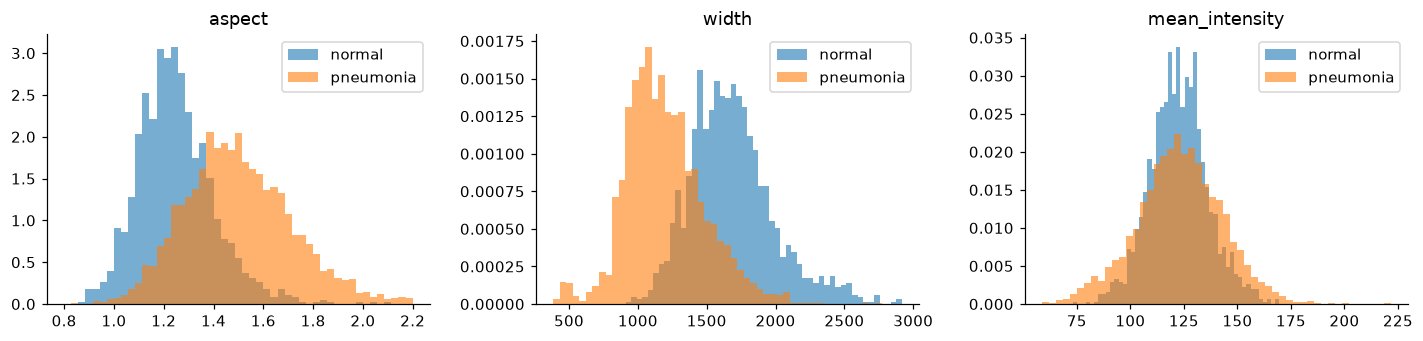
\includegraphics[width=.8\textwidth]{figures/a_acquisition_by_class.png}
\caption{Kermany acquisition properties by class: image size and file size separate the classes without looking at the lungs.}\label{fig:shortcut}
\end{figure}

\section{Method}

\subsection{Classifier (baseline and variants)}
\textbf{Baseline E1}: 1{,}000 real source images (500 per class), ImageNet-pretrained timm backbones (ResNet-18/50, DenseNet-121, EfficientNet-B0, ConvNeXt-T, ViT-S/16, Swin-T) with a single-logit head; grayscale replicated to three channels. CXR-pretrained weights were deliberately not used because they were trained on NIH data, i.e.\ on our external domain. Training: BCE, AdamW, bf16 autocast, all data and augmentation on the GPU, a fixed budget of 1{,}500 steps with validation every 50 steps, early stopping after 8 validations without improvement in validation BCE; the lowest-BCE checkpoint is kept; the decision threshold (Youden's $J$) is fixed on source validation.

\textbf{Hyper-parameters.} One Optuna study per architecture on E1 (TPE, median pruning, 25 trials; learning rate, weight decay, batch size, schedule, warm-up, head-LR multiplier, label smoothing, dropout, stochastic depth), objective = Kermany validation BCE. The best parameters are frozen for all experiments of that architecture and reused for CheXpert (not re-tuned; a limitation).

\textbf{Conventional augmentation.} E2: $\pm10^\circ$ rotation, $\pm6\%$ shift, $\pm10\%$ scale, brightness/contrast/gamma, no flips. Targeted variants: E2\_ERASE (random erasing + random border masking), E2\_ACQ (blur, noise, down/up-sampling), E2\_ROBUST (both), E2\_MIX (mixup), LP (frozen backbone).

\subsection{Generator}
Both generators use Stable Diffusion~1.5 \citep{rombach2022} with a LoRA adapter \citep{hu2022} (rank 16, $\alpha=16$, attention projections of the U-Net); the CLIP text encoder and the VAE stay frozen. Each training image is captioned with its class prompt (``a frontal cxr\_scan showing pneumonia, lung consolidation, radiograph'' or its normal counterpart). Sampling uses 30 denoising steps, a shared negative prompt, fixed seeds and balanced classes.
\begin{itemize}
\item \textbf{Study 1 (Kermany adapter, generative component of the team):} trained on Kermany training images, CFG 4.5; 4{,}000 normal + 1{,}000 pneumonia images at 512\,px.
\item \textbf{Study 2 (our CheXpert adapter):} the same training script (\code{scripts/\allowbreak{}generator/\allowbreak{}train\_\allowbreak{}lora.py}) on 9{,}968 CheXpert training images at 512\,px. v1 = the recipe as received (lr $2\cdot10^{-5}$, 2{,}500 steps $\times$ batch 4); v2 = lr $10^{-4}$, 7{,}500 steps (3 epochs, $\approx 2.3$\,h on 8\,GB with fp16 base weights and expandable CUDA segments); final = v2 sampled at CFG 2.5 (chosen by a guidance sweep). Further variants: rich report captions, rank 64, view captions, an ``obvious cases'' positive class and 29.5k training images (\S\ref{sec:gen}).
\end{itemize}

\textbf{Generator evaluation} (\code{scripts/\allowbreak{}generator/\allowbreak{}evaluate.py}): KID and precision/recall on ImageNet EfficientNet-B0 features against real training images; \emph{class signal} = the probability that a robust real-trained ``teacher'' (E2\_ERASE ensemble of EfficientNet-B0, DenseNet-121, ViT-S) assigns to synthetic normals and pneumonias, and the teacher's AUROC for the prompt label; \emph{memorisation} = cosine similarity of each synthetic image to its nearest real training image, flagged if it exceeds the largest similarity between two different real patients (0.926).

\subsection{Teacher labels}
TEACH replaces each synthetic image's prompt label by the teacher's probability (soft label, BCE). RTEACH applies the same teacher labels to \emph{real} images; it is the distillation control.

\section{Experimental protocol}
\label{sec:stats}
\begin{itemize}
\item \textbf{One variable at a time.} Every run shares the validation set, step budget, stopping rule, threshold rule and per-architecture hyper-parameters; only the training set changes. Matched real controls (R25 / R50 = +250 / +500 real images) accompany E3 / E4 (+250 / +500 synthetic).
\item \textbf{Selection never touches RSNA-test.} Checkpoints, thresholds and hyper-parameters are chosen on source validation. RSNA-dev was used once (choosing E2\_ERASE as the base of a follow-up series); every reported external number is on RSNA-test. In the synthetic-only arms marked ``V'', validation is synthetic too, so no real image enters the classifier pipeline.
\item \textbf{Statistics.} 3 seeds per configuration. Per-run 95\% CIs from a patient-clustered bootstrap (1{,}000 resamples); comparisons by paired bootstrap of 3-seed ensembles (2{,}000 resamples) plus per-seed mean and SD. Bootstrap CIs are tight ($\pm0.004$--$0.010$) but seed SD is 0.01--0.10, so $|\Delta|<0.03$ is treated as inconclusive.
\item \textbf{Tracking.} Every run logs parameters, curves, metrics, environment and git commit to MLflow; \code{scripts/\allowbreak{}catalogue.py} joins the 1{,}073 run directories with MLflow and recomputes the headline metric from saved predictions (\code{docs/\allowbreak{}CATALOGUE.md}).
\end{itemize}

\section{Results}
All values are view-balanced RSNA-test AUROC unless stated; ``$\Delta$'' is relative to E1 of the same architecture.

\subsection{Study 1: baselines and conventional augmentation}
\begin{table}[h]\centering\small
\resizebox{\textwidth}{!}{\begin{tabular}{lccccccc}\toprule
 & EffNet-B0 & ResNet-18 & ResNet-50 & DenseNet-121 & ConvNeXt-T & ViT-S & Swin-T\\\midrule
E1 & 0.736 & 0.771 & 0.747 & 0.787 & 0.713 & 0.692 & 0.698\\
E2 & 0.833 & 0.818 & 0.825 & 0.836 & 0.808 & 0.775 & 0.745\\
E2\_ERASE & \textbf{0.851} & \textbf{0.826} & \textbf{0.863} & \textbf{0.858} & 0.841 & \textbf{0.849} & 0.813\\
E2\_ACQ & 0.826 & 0.822 & 0.849 & 0.788 & \textbf{0.844} & 0.789 & \textbf{0.828}\\
LP (frozen) & 0.654 & 0.710 & 0.692 & 0.768 & 0.682 & 0.677 & 0.759\\\midrule
Kermany test, E1 & 0.937 & 0.945 & 0.947 & 0.932 & 0.867 & 0.866 & 0.878\\\bottomrule
\end{tabular}}
\caption{Study 1, mean of 3 seeds. Every model loses 0.15--0.20 AUROC from Kermany test to RSNA. Augmentation helps every architecture (+0.05 to +0.10, all CIs above 0); erasing is the best recipe for five of seven.}\label{tab:s1}
\end{table}
\textbf{Source validation is misleading:} Kermany validation BCE prefers E1 over E2 for 5 of 7 architectures, the opposite of the external result. \textbf{Variation matters more than size:} for EfficientNet-B0, augmentation on 1{,}000 images (+0.097) beats four times more real data (+0.049; FULL 0.785), and real data on top of augmentation adds almost nothing (FULL\_AUG 0.836).

\subsection{Study 1: synthetic augmentation (RQ1)}
\begin{table}[h]\centering\small
\begin{tabular}{lcccc}\toprule
 & +250 real & +500 real & \textbf{+250 synthetic} & \textbf{+500 synthetic}\\\midrule
EfficientNet-B0 & $+0.027$ & $+0.017$ & $\mathbf{-0.075}$ & $\mathbf{-0.103}$\\
ResNet-18 & $-0.021$ & $+0.003$ & $\mathbf{-0.081}$ & $\mathbf{-0.148}$\\
ResNet-50 & $+0.002$ & $+0.018$ & $\mathbf{-0.063}$ & $\mathbf{-0.082}$\\
DenseNet-121 & $+0.030$ & $+0.028$ & $\mathbf{-0.038}$ & $\mathbf{-0.019}$\\
ConvNeXt-T & $+0.015$ & $-0.017$ & $\mathbf{-0.041}$ & $\mathbf{-0.088}$\\
ViT-S & $+0.035$ & $+0.041$ & $\mathbf{-0.051}$ & $\mathbf{-0.090}$\\
Swin-T & $+0.051$ & $-0.056$ & $\mathbf{-0.104}$ & $\mathbf{-0.054}$\\\bottomrule
\end{tabular}
\caption{$\Delta$ vs E1, 3-seed ensembles; every synthetic CI is below 0. The same holds on top of E2\_ERASE (7 of 7 negative, $-0.030$ to $-0.145$).}\label{tab:e3e4}
\end{table}
Synthetic images hurt in \textbf{14 of 14} comparisons; 250--2{,}000 synthetic images give a similar penalty, and a classifier trained on 2{,}000 synthetic images only scores \textbf{0.525} (chance). Equalised preprocessing, four robust losses and quality-aware selection shrink the penalty at best by half; none turns it positive. The synthetic images carry little pathology: the teacher gives synthetic pneumonia a mean probability of 0.37 (real 0.96), and a linear probe separates synthetic from real perfectly (AUROC 1.000).

\subsection{Study 1: what causes the harm (RQ2)}
Each arm adds \emph{real} images that copy one property of the synthetic set, and we report the share of the synthetic penalty it reproduces (0 = like real images, 1 = like synthetic; median over EfficientNet-B0, ResNet-18, DenseNet-121 $\times$ two sizes): copied quality shortcut \textbf{0.08}; 30\% flipped labels \textbf{0.10}, 50--70\% $\approx$0.25; both 0.16; synthetic images with the 20\% anatomically worst removed \textbf{0.99}. \textbf{Counterfactual pairs} (a real film with only the lungs inpainted, once per prompt, so no hospital cue predicts the label) still hurt ($-0.03$ to $-0.16$), most when the two edits are nearly identical. Conclusion: the classifier learns whatever consistently separates the two prompts, which is a generator-specific texture, not disease.

\textbf{Teacher labels fix it.} Relabelling the same synthetic images with the teacher's probability removes the penalty in 6 of 6 cells (EfficientNet-B0 $+0.038$, ResNet-18 $-0.032$, DenseNet-121 $+0.053$ at +250, vs $-0.075$, $-0.081$, $-0.038$ with prompt labels). Teacher labels on extra \emph{real} images give similar gains ($+0.040$, $-0.023$, $+0.014$): mostly distillation.

\subsection{Study 2: changing the source}
Training on 1{,}000 CheXpert images instead of 1{,}000 Kermany images raises RSNA AUROC from 0.736 / 0.771 / 0.787 to \textbf{0.888 / 0.891 / 0.916} (EfficientNet-B0 / ResNet-18 / DenseNet-121; ensembles 0.92--0.94), \textbf{$+0.13$ on average}, the largest effect in the project. View-balanced training subsets change nothing ($|\Delta|\le0.01$). On CheXpert the classifier is near a plateau: 250 / 500 / 1{,}000 / 2{,}000 real images give 0.873 / 0.892 / 0.898 / 0.900 and all 9{,}968 give 0.930 (Fig.~\ref{fig:scaling}).

\subsection{Study 2: our generator (RQ3)}\label{sec:gen}
\begin{table}[h]\centering\small
\resizebox{\textwidth}{!}{\begin{tabular}{lccccc}\toprule
Generator & KID$\times$1000 $\downarrow$ & recall $\uparrow$ & teacher $p$(pneu) $\uparrow$ & synthetic-only RSNA & CheXpert test\\\midrule
real CheXpert (reference) & $\approx0$ & 0.83 & 0.74 & 0.900 (2k real) & 0.884\\\midrule
v1, recipe as received & 122 & 0.06 & 0.45 & 0.714 & 0.741\\
v2, lr $10^{-4}$, 7{,}500 steps & 213 & 0.35 & 0.13 & 0.833 & 0.776\\
\textbf{v2, CFG 2.5 (final)} & 103 & 0.62 & 0.37 & \textbf{0.833} & \textbf{0.807}\\
rich report captions & 79 & -- & 0.38 & 0.767 & 0.774\\
LoRA rank 64 & -- & -- & 0.42 & 0.764 & 0.794\\
view captions, 50/50 AP/PA & -- & -- & 0.33 & 0.814 & 0.809\\
obvious cases, 29k images & 64 & 0.63 & 0.31 & 0.744 & 0.761\\
3$\times$ data (29.5k), 15k steps & 82 & 0.57 & 0.26 & 0.756 & 0.769\\\bottomrule
\end{tabular}}
\caption{Generator versions (2{,}000 images; synthetic-only rows from v2 on use synthetic validation). Mean of 3 architectures $\times$ 3 seeds.}\label{tab:gen}
\end{table}

\begin{figure}[h]\centering
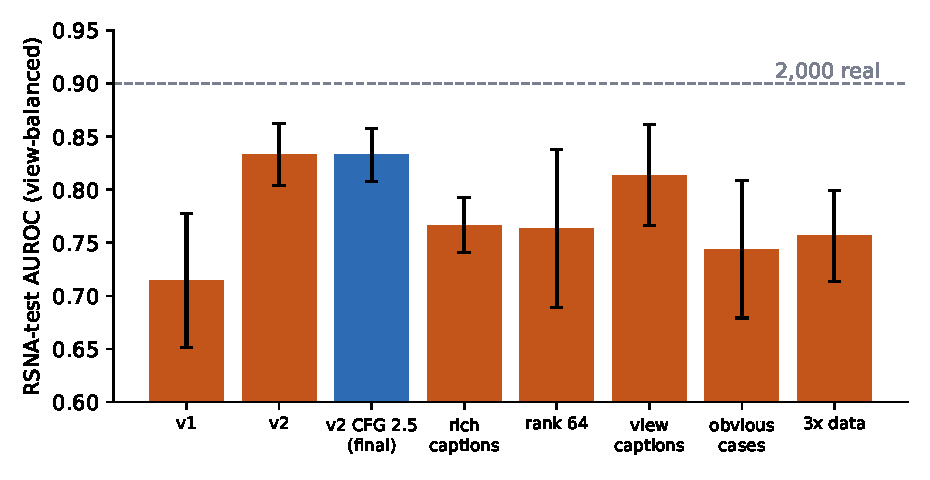
\includegraphics[width=.72\textwidth]{figures/s2_generator_versions.pdf}
\caption{Synthetic-only RSNA AUROC per generator version (2{,}000 images, error bars: SD over 3 architectures $\times$ 3 seeds). Dashed: 2{,}000 real images.}\label{fig:gen}
\end{figure}

Training longer at a normal LoRA learning rate halved the gap to real data (0.714 $\rightarrow$ 0.833); the guidance sweep (1.5 / 2.5 / 3.5 / 4.5) showed that CFG 2.5 keeps the class signal of 4.5 with half the KID gap and higher recall. After that, \textbf{every lever improved realism and none improved the classifier}: KID fell from 103 to 64--82 while synthetic-only AUROC fell to 0.74--0.77. The teacher's $p$(pneumonia) on synthetic positives (0.26--0.42 vs 0.74 real) tracks downstream usefulness; KID does not. A VAE round trip of real films keeps the teacher's signal (AUROC 0.902 $\rightarrow$ 0.892), so the loss happens in the denoiser and its conditioning. The 29.5k-image generator (pass mark: clearly above 0.833) scored 0.756 and was rejected.

\begin{figure}[h]\centering
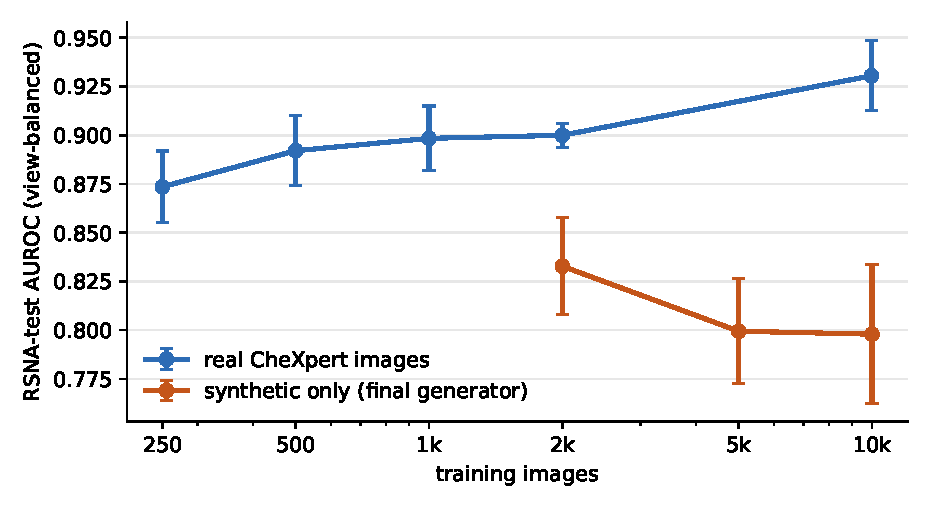
\includegraphics[width=.72\textwidth]{figures/s2_scaling.pdf}
\caption{Replacement test. Real CheXpert images (blue) vs synthetic-only training with the final generator (orange). 2{,}000 synthetic images (0.833) are worth less than 250 real ones (0.873); 5k and 10k do not help.}\label{fig:scaling}
\end{figure}

\textbf{More is not better.} 5{,}000 and 10{,}000 synthetic images give 0.800 and 0.798; synthetic validation AUROC keeps rising (0.92--0.96) because the classifier separates the generator's two prompts ever better, a skill that does not transfer. Mixing synthetic into real data costs $\approx-0.02$ even with only 250 real images (0.857 vs 0.873).

\subsection{Final controls: images or teacher?}
\begin{figure}[h]\centering
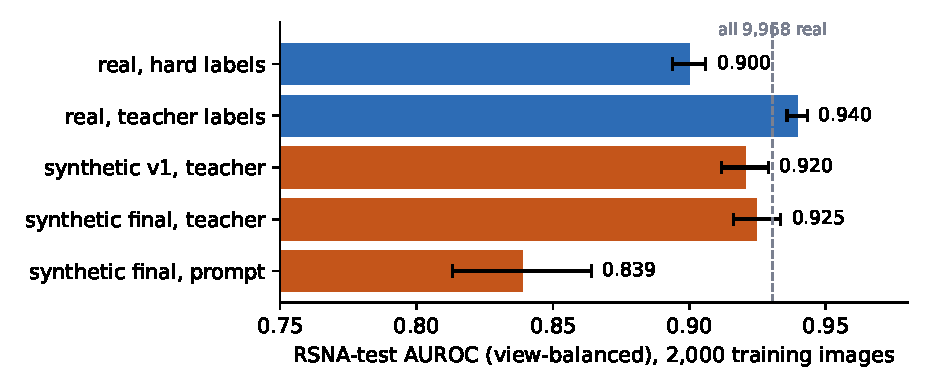
\includegraphics[width=.72\textwidth]{figures/s2_final_controls.pdf}
\caption{2{,}000 training images each, real CheXpert validation. Real images unseen by the teacher (subset ranks 1{,}000--1{,}999) with teacher labels beat synthetic images with teacher labels for every architecture.}\label{fig:controls}
\end{figure}
Synthetic-only with teacher labels reaches 0.920 (v1 images) and 0.925 (final images), far above prompt labels (0.839), and even above 2{,}000 real images with hard labels (0.900). The control resolves it: 2{,}000 \emph{real} images the teacher never saw, with the same teacher labels, reach \textbf{0.940} (per architecture 0.943 / 0.936 / 0.939 vs 0.931 / 0.913 / 0.930 synthetic, seed SD $\le0.004$), above all 9{,}968 real images with hard labels (0.930). A better generator adds only $+0.005$ under teacher labels but $+0.12$ under prompt labels. The strong synthetic result is therefore distillation of a model trained on real patients, transmitted through synthetic images.

\subsection{Comparison with Ktena et al.\ (RQ4)}
Following their recipe on our runs (1{,}000 real CheXpert images + synthetic images with prompt labels), RSNA AUROC is 0.891 / 0.896 (+250 / +500) and 0.881 (+2{,}000) vs 0.898 for real alone; the sex AUROC gap is 0.003--0.011 in every arm, i.e.\ there is no fairness gap for synthetic data to close. The differences to their setup are large: 201k vs $\approx$10k labelled images behind the generator (20$\times$); a pixel-space diffusion model trained on X-rays vs a LoRA on a natural-image latent model; conditioning on the full label vector and sampling with the real label mix vs one text prompt per class. Our experiments exclude the cheap explanations (quantity of synthetic images, the view shortcut, LoRA capacity, the VAE, the validation scheme); what remains is what our hardware could not provide.

\subsection{Error analysis}
On RSNA, Kermany-trained models (notebook 05) mostly fail in three ways: (1) normal AP/portable films flagged as pneumonia (E1 specificity on AP normals $\approx0.24$; Grad-CAM shows diffuse heat plus ``PORTABLE'' markers); (2) focal adult consolidations on clean PA films missed; (3) other diseases (\emph{Not Normal}) called pneumonia (median score 0.98). The first two are absent from Kermany by construction, which is why more Kermany-like data, real or synthetic, cannot fix them and why the source switch helps. Sex differences are small ($\le0.03$); the paediatric part of RSNA is not easier, so the shift is hospital and acquisition more than age.

\section{Optimisation and resources}
\label{sec:opt}
All measurements on the project hardware (one RTX 3060 Ti 8\,GB, 12-core CPU) with \code{scripts/\allowbreak{}optimize\_\allowbreak{}bench.py}, using the CheXpert E2\_ERASE models (seed 0) and the same quality metric as everywhere else, recomputed for every variant (\code{reports/\allowbreak{}results/\allowbreak{}optimize\_\allowbreak{}bench.csv}).

\begin{table}[h]\centering\small
\begin{tabular}{lrrrrrr}\toprule
 & params & size & \multicolumn{2}{c}{GPU images/s} & CPU latency & RSNA AUROC\\
Model & (M) & (MB) & fp32 & bf16 & (ms, batch 1) & fp32 / bf16\\\midrule
EfficientNet-B0 & 4.0 & 15.6 & 780 & 1{,}515 & 11.4 & 0.9268 / 0.9263\\
ResNet-18 & 11.2 & 42.7 & 2{,}202 & 4{,}095 & 13.4 & 0.9184 / 0.9190\\
DenseNet-121 & 7.0 & 27.1 & 670 & 1{,}373 & 29.6 & 0.9153 / 0.9152\\
ViT-S/16 & 21.7 & 82.7 & 734 & 1{,}844 & 43.0 & 0.9299 / 0.9300\\\bottomrule
\end{tabular}
\caption{Size, GPU throughput (batch 128, end to end including host-to-device transfer, 17k RSNA images) and CPU latency (median of 50 runs, 4 threads, $224{\times}224$).}\label{tab:opt}
\end{table}

\paragraph{Optimisation 1: bf16 mixed precision (used for all training and evaluation).} Throughput rises $1.9$--$2.5\times$ and peak GPU memory falls by 16\% (ViT-S) to 46\% (EfficientNet-B0), while AUROC changes by at most $0.0006$, far below the $0.03$ noise threshold. This is what made $\approx$1{,}100 runs fit on one consumer GPU: the median CheXpert run trains in 88\,s (IQR 45--117\,s).

\paragraph{Optimisation 2: int8 dynamic quantisation for CPU deployment (ViT-S).} Quantising the Linear layers shrinks the model from 82.7 to 22.0\,MB ($-73\%$) and cuts CPU latency from 43.0 to 29.8\,ms ($-31\%$), at a cost of $-0.004$ AUROC (0.9299 $\rightarrow$ 0.9259), within seed noise. For the convolutional models the same method does nothing useful (their compute is in convolutions), so the demo uses EfficientNet-B0, which is already the fastest on CPU (11.4\,ms) and among the most accurate.

\paragraph{Trade-off: seed ensembles.} Averaging three seeds raises AUROC by $+0.007$ (ViT-S) to $+0.029$ (EfficientNet-B0) at $3\times$ the inference cost (0.9055 $\rightarrow$ 0.9350 for EfficientNet-B0). Even three EfficientNet-B0 models (34\,ms on CPU) are faster than one ViT-S. We report single models as the headline and ensembles as a variant.

\paragraph{Generator costs.} LoRA training at 512\,px ran out of memory on 8\,GB until the base weights were loaded in fp16 and PyTorch's expandable memory segments were enabled (no recipe change); it then runs at 1.1\,s per step (v2: $\approx$2.3\,h). Sampling takes $\approx$2.4\,s per image (30 steps), so the 10{,}000-image set took $\approx$7\,h. LoRA (rank 16) instead of full fine-tuning is itself the main resource decision: it trains $\sim$3M parameters instead of 860M and fits the GPU.

\section{Responsible AI, risks and limitations}
\begin{table}[h]\centering\small
\begin{tabularx}{\textwidth}{lYY}\toprule
Risk & Where it shows up & Mitigation and check\\\midrule
Silent failure at other hospitals & $-0.15$ to $-0.20$ AUROC from Kermany test to RSNA & external hospital as primary endpoint; per-view reporting; demo shows the training population and external metrics\\
Shortcut learning & file size, view, markers & full-FOV resizing; metadata-only probe; view-balanced metric; Grad-CAM border analysis; demo blur/contrast stress test\\
Synthetic data teaches generator artefacts & 14 of 14 negative comparisons & matched real controls; teacher-signal check of every generator \emph{before} training classifiers; recommendation not to train on prompt labels\\
Privacy / memorisation & generators trained on patient images & nearest-neighbour check: 0 of 10{,}000 synthetic images closer to a training image than two real patients (max 0.917 vs 0.926)\\
Population bias & Kermany: Chinese children; RSNA: US adults & subgroup analysis by view, sex, age; sex AUROC gap 0.003--0.011 in study 2\\
Over-trust & a score read as a diagnosis & research-only labelling in the demo, no treatment advice\\\bottomrule
\end{tabularx}
\caption{Risks, mitigations and the checks performed.}
\end{table}
\textbf{Limitations.} One 8\,GB GPU: LoRA only, no X-ray-native diffusion model; hyper-parameters tuned on Kermany and reused for CheXpert; one external hospital (plus CheXpert test as a second check); fairness measured for sex only; 224\,px resolution; three seeds give limited power below $|\Delta|=0.03$; teacher-label training still requires a model trained on real patients. Demo example images were chosen to illustrate typical cases and are not evidence.

\section{Conclusions}
\begin{enumerate}
\item[RQ1] \textbf{No.} Prompt-labelled synthetic images from a Kermany-trained generator lowered external AUROC in 14 of 14 comparisons, while matched real images were neutral or positive.
\item[RQ2] Not the copied shortcut (share 0.08), label noise ($\le0.25$) or anatomy (0.99), but a \textbf{generator-specific class cue} learned through prompt labels; soft teacher labels remove it.
\item[RQ3] \textbf{Not at our scale.} Our best generator's 2{,}000 images (0.833) are worth less than 250 real images (0.873); more synthetic data does not help; no memorisation was found. With teacher labels synthetic images carry a real model's knowledge nearly as well as real images ($-0.015$), which is distillation, not replacement.
\item[RQ4] Twenty times less generator data, a natural-image prior and one-bit conditioning; the cheaper explanations were ruled out experimentally.
\end{enumerate}
Practical lessons: the source dataset matters more than its size; evaluate a generator by how much disease a real-trained model sees in its output, not by realism scores; and never select recipes on the source hospital alone.

\section{Reproducibility}
Code: \code{cxr/\allowbreak{}} (library), \code{scripts/\allowbreak{}} (CLI and queues), \code{notebooks/\allowbreak{}} (generated from \code{notebooks/\allowbreak{}\_\allowbreak{}build/\allowbreak{}}). Environments: \code{requirements.txt} (classifiers) and \code{requirements-gen.txt} (generator). Data access: Kermany (Kaggle, CC BY 4.0), RSNA (Kaggle / RSNA challenge), CheXpert Plus (Stanford AIMI research-use agreement via Redivis; \code{scripts/\allowbreak{}chexpert/\allowbreak{}fetch.py}); no images are redistributed. Main experiments: \code{scripts/\allowbreak{}pipeline.sh} (study 1), \code{scripts/\allowbreak{}queue\_\allowbreak{}cx.sh}, \code{scripts/\allowbreak{}queue\_\allowbreak{}gen\_\allowbreak{}cx.sh}, \code{scripts/\allowbreak{}queue\_\allowbreak{}gen\_\allowbreak{}v2*.sh}, \code{scripts/\allowbreak{}queue\_\allowbreak{}gen\_\allowbreak{}scale.sh}, \code{scripts/\allowbreak{}queue\_\allowbreak{}final.sh} (study 2); tables: \code{scripts/\allowbreak{}catalogue.py}, \code{scripts/\allowbreak{}generator/\allowbreak{}syn\_\allowbreak{}only\_\allowbreak{}table.py}; resources: \code{scripts/\allowbreak{}optimize\_\allowbreak{}bench.py}. All queues are resumable and skip finished runs. Full experiment index: \code{docs/\allowbreak{}CATALOGUE.md}.

\section{Individual contributions}
Full table with links to files, experiments and slides: \code{docs/CONTRIBUTIONS.md}.

\begin{table}[h]\centering\small
\begin{tabularx}{\textwidth}{lYY}\toprule
Member & Work & Evidence\\\midrule
Trubarov Nikita & prediction component: data pipeline, splits and leakage checks, classifier training and HPO, all experiments of studies 1 and 2, CheXpert generator training and evaluation, analyses, demo, report & \code{cxr/\allowbreak{}}, \code{scripts/\allowbreak{}}, notebooks 01--07, \code{docs/\allowbreak{}RESEARCH\_\allowbreak{}PIVOT.md}, \code{docs/\allowbreak{}CATALOGUE.md}, \S\S3--7\\
Yerlan Kubesov & generative component: Stable Diffusion 1.5 LoRA training script and recipe, the Kermany generator and its 5{,}000 synthetic images & \code{scripts/\allowbreak{}generator/\allowbreak{}train\_\allowbreak{}lora.py}, \code{data/\allowbreak{}synthetic/\allowbreak{}sd\_\allowbreak{}lora/\allowbreak{}}, \S4.2\\\bottomrule
\end{tabularx}
\end{table}

\appendix
\section{Borrowed components and AI tools}
\textbf{Pretrained models and libraries.} Stable Diffusion~1.5 weights (generator base); timm ImageNet backbones; torchxrayvision PSPNet (anatomy scoring only); PyTorch, diffusers, PEFT, transformers, Optuna, MLflow, scikit-learn, Streamlit. The LoRA training script is the generative component's, vendored with three changes (fp16 base weights, seed argument, model id).

\textbf{AI assistants.} Claude (Anthropic) was used through Claude Code as a coding and analysis assistant: writing and refactoring scripts, orchestrating experiment queues on the GPU workstation, computing result tables, drafting documentation, this report and the slides. Verification by the team: every reported number is recomputed by scripts from saved per-run predictions (\code{scripts/\allowbreak{}catalogue.py}, \code{*\_\allowbreak{}compare.py}) and is traceable to MLflow runs; claims were revised when controls contradicted them (e.g.\ the withdrawn ``harmonisation removes the penalty'' result, the corrected TEACH comparison); code and text were reviewed by the team before submission. The Kermany generator (study 1) was produced with the original LoRA training script; no AI-assistant use was reported for it.

\setlength{\bibhang}{0.5in}\setlength{\bibsep}{3pt}
\small
\renewcommand{\refname}{References}
\begin{thebibliography}{}
\bibitem[{Akiba et~al.}(2019)]{akiba2019} Akiba, T., Sano, S., Yanase, T., Ohta, T., \& Koyama, M. (2019). Optuna: A next-generation hyperparameter optimization framework. In \textit{Proceedings of the 25th ACM SIGKDD International Conference on Knowledge Discovery \& Data Mining} (pp. 2623--2631). ACM. \url{https://doi.org/10.1145/3292500.3330701}
\bibitem[{Bi\'nkowski et~al.}(2018)]{binkowski2018} Bi\'nkowski, M., Sutherland, D. J., Arbel, M., \& Gretton, A. (2018). Demystifying MMD GANs. In \textit{International Conference on Learning Representations}. \url{https://doi.org/10.48550/arXiv.1801.01401}
\bibitem[{Carlini et~al.}(2023)]{carlini2023} Carlini, N., Hayes, J., Nasr, M., Jagielski, M., Sehwag, V., Tram\`er, F., Balle, B., Ippolito, D., \& Wallace, E. (2023). Extracting training data from diffusion models. In \textit{32nd USENIX Security Symposium} (pp. 5253--5270). USENIX Association. \url{https://doi.org/10.48550/arXiv.2301.13188}
\bibitem[{Chambon et~al.}(2022)]{chambon2022} Chambon, P., Bluethgen, C., Delbrouck, J.-B., Van der Sluijs, R., Po\l{}acin, M., Zambrano Chaves, J. M., Abraham, T. M., Purohit, S., Langlotz, C. P., \& Chaudhari, A. (2022). \textit{RoentGen: Vision-language foundation model for chest X-ray generation} [Preprint]. arXiv. \url{https://doi.org/10.48550/arXiv.2211.12737}
\bibitem[{Cohen et~al.}(2022)]{cohen2022} Cohen, J. P., Viviano, J. D., Bertin, P., Morrison, P., Torabian, P., Guarrera, M., Lungren, M. P., Chaudhari, A., Brooks, R., Hashir, M., \& Bertrand, H. (2022). TorchXRayVision: A library of chest X-ray datasets and models. In \textit{Proceedings of the 5th International Conference on Medical Imaging with Deep Learning} (Proceedings of Machine Learning Research, Vol. 172, pp. 231--249). \url{https://doi.org/10.48550/arXiv.2111.00595}
\bibitem[{DeGrave et~al.}(2021)]{degrave2021} DeGrave, A. J., Janizek, J. D., \& Lee, S.-I. (2021). AI for radiographic COVID-19 detection selects shortcuts over signal. \textit{Nature Machine Intelligence}, \textit{3}(7), 610--619. \url{https://doi.org/10.1038/s42256-021-00338-7}
\bibitem[{Geirhos et~al.}(2020)]{geirhos2020} Geirhos, R., Jacobsen, J.-H., Michaelis, C., Zemel, R., Brendel, W., Bethge, M., \& Wichmann, F. A. (2020). Shortcut learning in deep neural networks. \textit{Nature Machine Intelligence}, \textit{2}(11), 665--673. \url{https://doi.org/10.1038/s42256-020-00257-z}
\bibitem[{He et~al.}(2023)]{he2023} He, R., Sun, S., Yu, X., Xue, C., Zhang, W., Torr, P., Bai, S., \& Qi, X. (2023). Is synthetic data from generative models ready for image recognition? In \textit{International Conference on Learning Representations}. \url{https://doi.org/10.48550/arXiv.2210.07574}
\bibitem[{Hinton et~al.}(2015)]{hinton2015} Hinton, G., Vinyals, O., \& Dean, J. (2015). \textit{Distilling the knowledge in a neural network} [Preprint]. arXiv. \url{https://doi.org/10.48550/arXiv.1503.02531}
\bibitem[{Ho \& Salimans}(2021)]{ho2021} Ho, J., \& Salimans, T. (2021). Classifier-free diffusion guidance. In \textit{NeurIPS 2021 Workshop on Deep Generative Models and Downstream Applications}. \url{https://doi.org/10.48550/arXiv.2207.12598}
\bibitem[{Hu et~al.}(2022)]{hu2022} Hu, E. J., Shen, Y., Wallis, P., Allen-Zhu, Z., Li, Y., Wang, S., Wang, L., \& Chen, W. (2022). LoRA: Low-rank adaptation of large language models. In \textit{International Conference on Learning Representations}. \url{https://doi.org/10.48550/arXiv.2106.09685}
\bibitem[{Irvin et~al.}(2019)]{irvin2019} Irvin, J., Rajpurkar, P., Ko, M., Yu, Y., Ciurea-Ilcus, S., Chute, C., Marklund, H., Haghgoo, B., Ball, R., Shpanskaya, K., Seekins, J., Mong, D. A., Halabi, S. S., Sandberg, J. K., Jones, R., Larson, D. B., Langlotz, C. P., Patel, B. N., Lungren, M. P., \& Ng, A. Y. (2019). CheXpert: A large chest radiograph dataset with uncertainty labels and expert comparison. \textit{Proceedings of the AAAI Conference on Artificial Intelligence}, \textit{33}(1), 590--597. \url{https://doi.org/10.1609/aaai.v33i01.3301590}
\bibitem[{Kermany et~al.}(2018)]{kermany2018} Kermany, D. S., Goldbaum, M., Cai, W., Valentim, C. C. S., Liang, H., Baxter, S. L., McKeown, A., Yang, G., Wu, X., Yan, F., Dong, J., Prasadha, M. K., Pei, J., Ting, M. Y. L., Zhu, J., Li, C., Hewett, S., Dong, J., Ziyar, I., \ldots\ Zhang, K. (2018). Identifying medical diagnoses and treatable diseases by image-based deep learning. \textit{Cell}, \textit{172}(5), 1122--1131.e9. \url{https://doi.org/10.1016/j.cell.2018.02.010}
\bibitem[{Ktena et~al.}(2024)]{ktena2024} Ktena, I., Wiles, O., Albuquerque, I., Rebuffi, S.-A., Tanno, R., Guha Roy, A., Azizi, S., Belgrave, D., Kohli, P., Cemgil, T., Karthikesalingam, A., \& Gowal, S. (2024). Generative models improve fairness of medical classifiers under distribution shifts. \textit{Nature Medicine}, \textit{30}(4), 1166--1173. \url{https://doi.org/10.1038/s41591-024-02838-6}
\bibitem[{Kynk\"a\"anniemi et~al.}(2019)]{kynkaanniemi2019} Kynk\"a\"anniemi, T., Karras, T., Laine, S., Lehtinen, J., \& Aila, T. (2019). Improved precision and recall metric for assessing generative models. In \textit{Advances in Neural Information Processing Systems} (Vol. 32). \url{https://doi.org/10.48550/arXiv.1904.06991}
\bibitem[{Packh\"auser et~al.}(2023)]{packhauser2023} Packh\"auser, K., Folle, L., Thamm, F., \& Maier, A. (2023). Generation of anonymous chest radiographs using latent diffusion models for training thoracic abnormality classification systems. In \textit{2023 IEEE 20th International Symposium on Biomedical Imaging (ISBI)} (pp. 1--5). IEEE. \url{https://doi.org/10.1109/ISBI53787.2023.10230346}
\bibitem[{Rombach et~al.}(2022)]{rombach2022} Rombach, R., Blattmann, A., Lorenz, D., Esser, P., \& Ommer, B. (2022). High-resolution image synthesis with latent diffusion models. In \textit{2022 IEEE/CVF Conference on Computer Vision and Pattern Recognition (CVPR)} (pp. 10674--10685). IEEE. \url{https://doi.org/10.1109/CVPR52688.2022.01042}
\bibitem[{Shih et~al.}(2019)]{shih2019} Shih, G., Wu, C. C., Halabi, S. S., Kohli, M. D., Prevedello, L. M., Cook, T. S., Sharma, A., Amorosa, J. K., Arteaga, V., Galperin-Aizenberg, M., Gill, R. R., Godoy, M. C. B., Hobbs, S., Jeudy, J., Laroia, A., Shah, P. N., Vummidi, D., Yaddanapudi, K., \& Stein, A. (2019). Augmenting the National Institutes of Health chest radiograph dataset with expert annotations of possible pneumonia. \textit{Radiology: Artificial Intelligence}, \textit{1}(1), Article e180041. \url{https://doi.org/10.1148/ryai.2019180041}
\bibitem[{Wang et~al.}(2017)]{wang2017} Wang, X., Peng, Y., Lu, L., Lu, Z., Bagheri, M., \& Summers, R. M. (2017). ChestX-ray8: Hospital-scale chest X-ray database and benchmarks on weakly-supervised classification and localization of common thorax diseases. In \textit{2017 IEEE Conference on Computer Vision and Pattern Recognition (CVPR)} (pp. 3462--3471). IEEE. \url{https://doi.org/10.1109/CVPR.2017.369}
\bibitem[{Zech et~al.}(2018)]{zech2018} Zech, J. R., Badgeley, M. A., Liu, M., Costa, A. B., Titano, J. J., \& Oermann, E. K. (2018). Variable generalization performance of a deep learning model to detect pneumonia in chest radiographs: A cross-sectional study. \textit{PLOS Medicine}, \textit{15}(11), Article e1002683. \url{https://doi.org/10.1371/journal.pmed.1002683}
\bibitem[{Zhong et~al.}(2020)]{zhong2020} Zhong, Z., Zheng, L., Kang, G., Li, S., \& Yang, Y. (2020). Random erasing data augmentation. \textit{Proceedings of the AAAI Conference on Artificial Intelligence}, \textit{34}(7), 13001--13008. \url{https://doi.org/10.1609/aaai.v34i07.7000}
\end{thebibliography}
\end{document}
